% Why this is not the usual random-effects fit: the patients are never observed.
% Left  -- the standard setting: per-patient observations, likelihood factors.
% Right -- here: the patients are latent, and what crosses the boundary is a
%          handful of numbers a paper printed.
%
%   compile:  pdflatex why_hard.tex
%
\documentclass[border=10pt]{standalone}
\usepackage{lmodern}
\usepackage{amsmath}
\usepackage{amssymb}
\usepackage{tikz}
\usetikzlibrary{arrows.meta,positioning,calc}
% Shared palette for the population-model figures.
%   ink      body / structure
%   popcol   the patient cloud and anything predicted from it
%   mechcol  the simulator and species-level quantities
%   msrcol   the measurement map (readout-level: gamma, kappa)
%   datacol  reported rows
\definecolor{ink}{HTML}{3A3A3A}
\definecolor{popcol}{HTML}{3B4AA6}
\definecolor{mechcol}{HTML}{2E7D5B}
\definecolor{msrcol}{HTML}{EB811B}
\definecolor{datacol}{HTML}{8C3B4A}


% standing person: #1 x, #2 y, #3 colour
\newcommand{\person}[3]{%
  \fill[#3] (#1,#2+0.40) circle (0.075);
  \fill[#3] (#1,#2+0.16) ellipse (0.10 and 0.145);}

\begin{document}
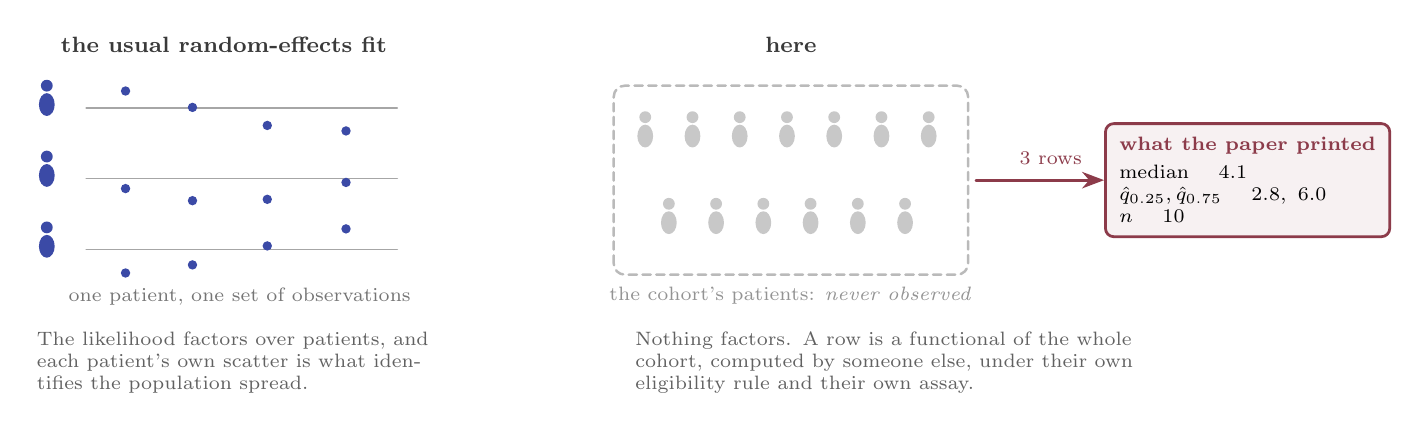
\begin{tikzpicture}[
  font=\sffamily, >=Stealth, line cap=round, line join=round,
  ttl/.style={font=\footnotesize\bfseries, anchor=south},
  figcap/.style={font=\scriptsize, text=ink!80, align=left, anchor=north west},
  card/.style={draw=datacol, fill=datacol!7, rounded corners=3pt,
               line width=1pt, inner sep=5pt, align=left, font=\scriptsize}]

% ==================================================== left: the usual setting
\begin{scope}[shift={(0,0)}]
  \node[ttl, ink] at (2.5,2.55) {the usual random-effects fit};
  \foreach \k/\y in {1/1.85, 2/0.95, 3/0.05}{
    \person{0.25}{\y}{popcol}
    \draw[ink!45, line width=0.6pt] (0.75,\y+0.12) -- (4.7,\y+0.12);
    \foreach \t in {1.25,2.10,3.05,4.05}
      \fill[popcol] (\t,{\y+0.12+0.30*sin(\t*52+\k*70)}) circle (1.7pt);}
  \node[ink!70, font=\scriptsize, anchor=north] at (2.7,-0.20)
    {one patient, one set of observations};
\end{scope}
\node[figcap, text width=50mm] at (0,-0.75)
  {The likelihood factors over patients, and each patient's own scatter is what
   identifies the population spread.};

% ==================================================== right: here
\begin{scope}[shift={(7.6,0)}]
  \node[ttl, ink] at (2.1,2.55) {here};

  % the latent cohort
  \draw[ink!35, densely dashed, rounded corners=4pt, line width=0.9pt]
    (-0.15,-0.15) rectangle (4.35,2.25);
  \foreach \x in {0.25,0.85,1.45,2.05,2.65,3.25,3.85}{
    \person{\x}{1.45}{ink!28}}
  \foreach \x in {0.55,1.15,1.75,2.35,2.95,3.55}{
    \person{\x}{0.35}{ink!28}}
  \node[ink!55, font=\scriptsize, anchor=north] at (2.1,-0.18)
    {the cohort's patients: \emph{never observed}};

  % what actually crosses the boundary
  \node[card] (c) at (7.9,1.05)
    {\textcolor{datacol}{\textbf{what the paper printed}}\\[2pt]
     median \quad $4.1$\\
     $\hat q_{0.25},\hat q_{0.75}$ \quad $2.8,\ 6.0$\\
     $n$ \quad $10$};
  \draw[-{Stealth[length=2.8mm]}, datacol, line width=1pt]
    (4.45,1.05) -- (c.west);
  \node[datacol, font=\scriptsize, anchor=south] at (5.4,1.12) {3 rows};
\end{scope}
\node[figcap, text width=68mm] at (7.6,-0.75)
  {Nothing factors. A row is a functional of the whole cohort, computed by
   someone else, under their own eligibility rule and their own assay.};

\end{tikzpicture}
\end{document}
